%%%%%%%%%%%%%%%%%%%%% {{{
%%Options for presentations (in-class) and handouts (e.g. print).
\documentclass[pdf,9pt]{beamer}
% \documentclass[pdf,9pt]{beamer}


%%%%%%%%%%%%%%%%%%%%%%
%Change this for different slides so it appears in bar
\usepackage{authoraftertitle}
\date{Chapter 8. Orthogonality \\ \S  8-4. QR Factorization}

%%%%%%%%%%%%%%%%%%%%%%
%% Upload common style file
\usepackage{LyryxLAWASlidesStyle}

\begin{document}

%%%%%%%%%%%%%%%%%%%%%%%
%% Title Page and Copyright Common to All Slides

%Title Page
\input frontmatter/titlepage.tex

%LOTS Page
\input frontmatter/lyryxopentexts.tex

%Copyright Page
\input frontmatter/copyright.tex

%%%%%%%%%%%%%%%%%%%%%%%%% }}}
%-------------- start slide -------------------------------%{{{ 2

\begin{frame}[fragile]
   \tableofcontents
\end{frame}
%-------------- end slide -------------------------------%}}}
\section[\textcolor{yellow}{}]{\textcolor{yellow}{QR Factorization}}
%-------------- start slide -----------------------------% {{{ 3
\frame{
\frametitle{The $QR$ Factorization}
\pause
\begin{definition}
    Let $A$ be a real $m \times n$ matrix. Then a \alert{$QR$ factorization} of $A$ can be written as \[
    A = QR
    \]
    where $Q$ is an orthogonal matrix and $R$ is an upper (or right) triangular matrix.
\end{definition}
\vfill
\begin{center} 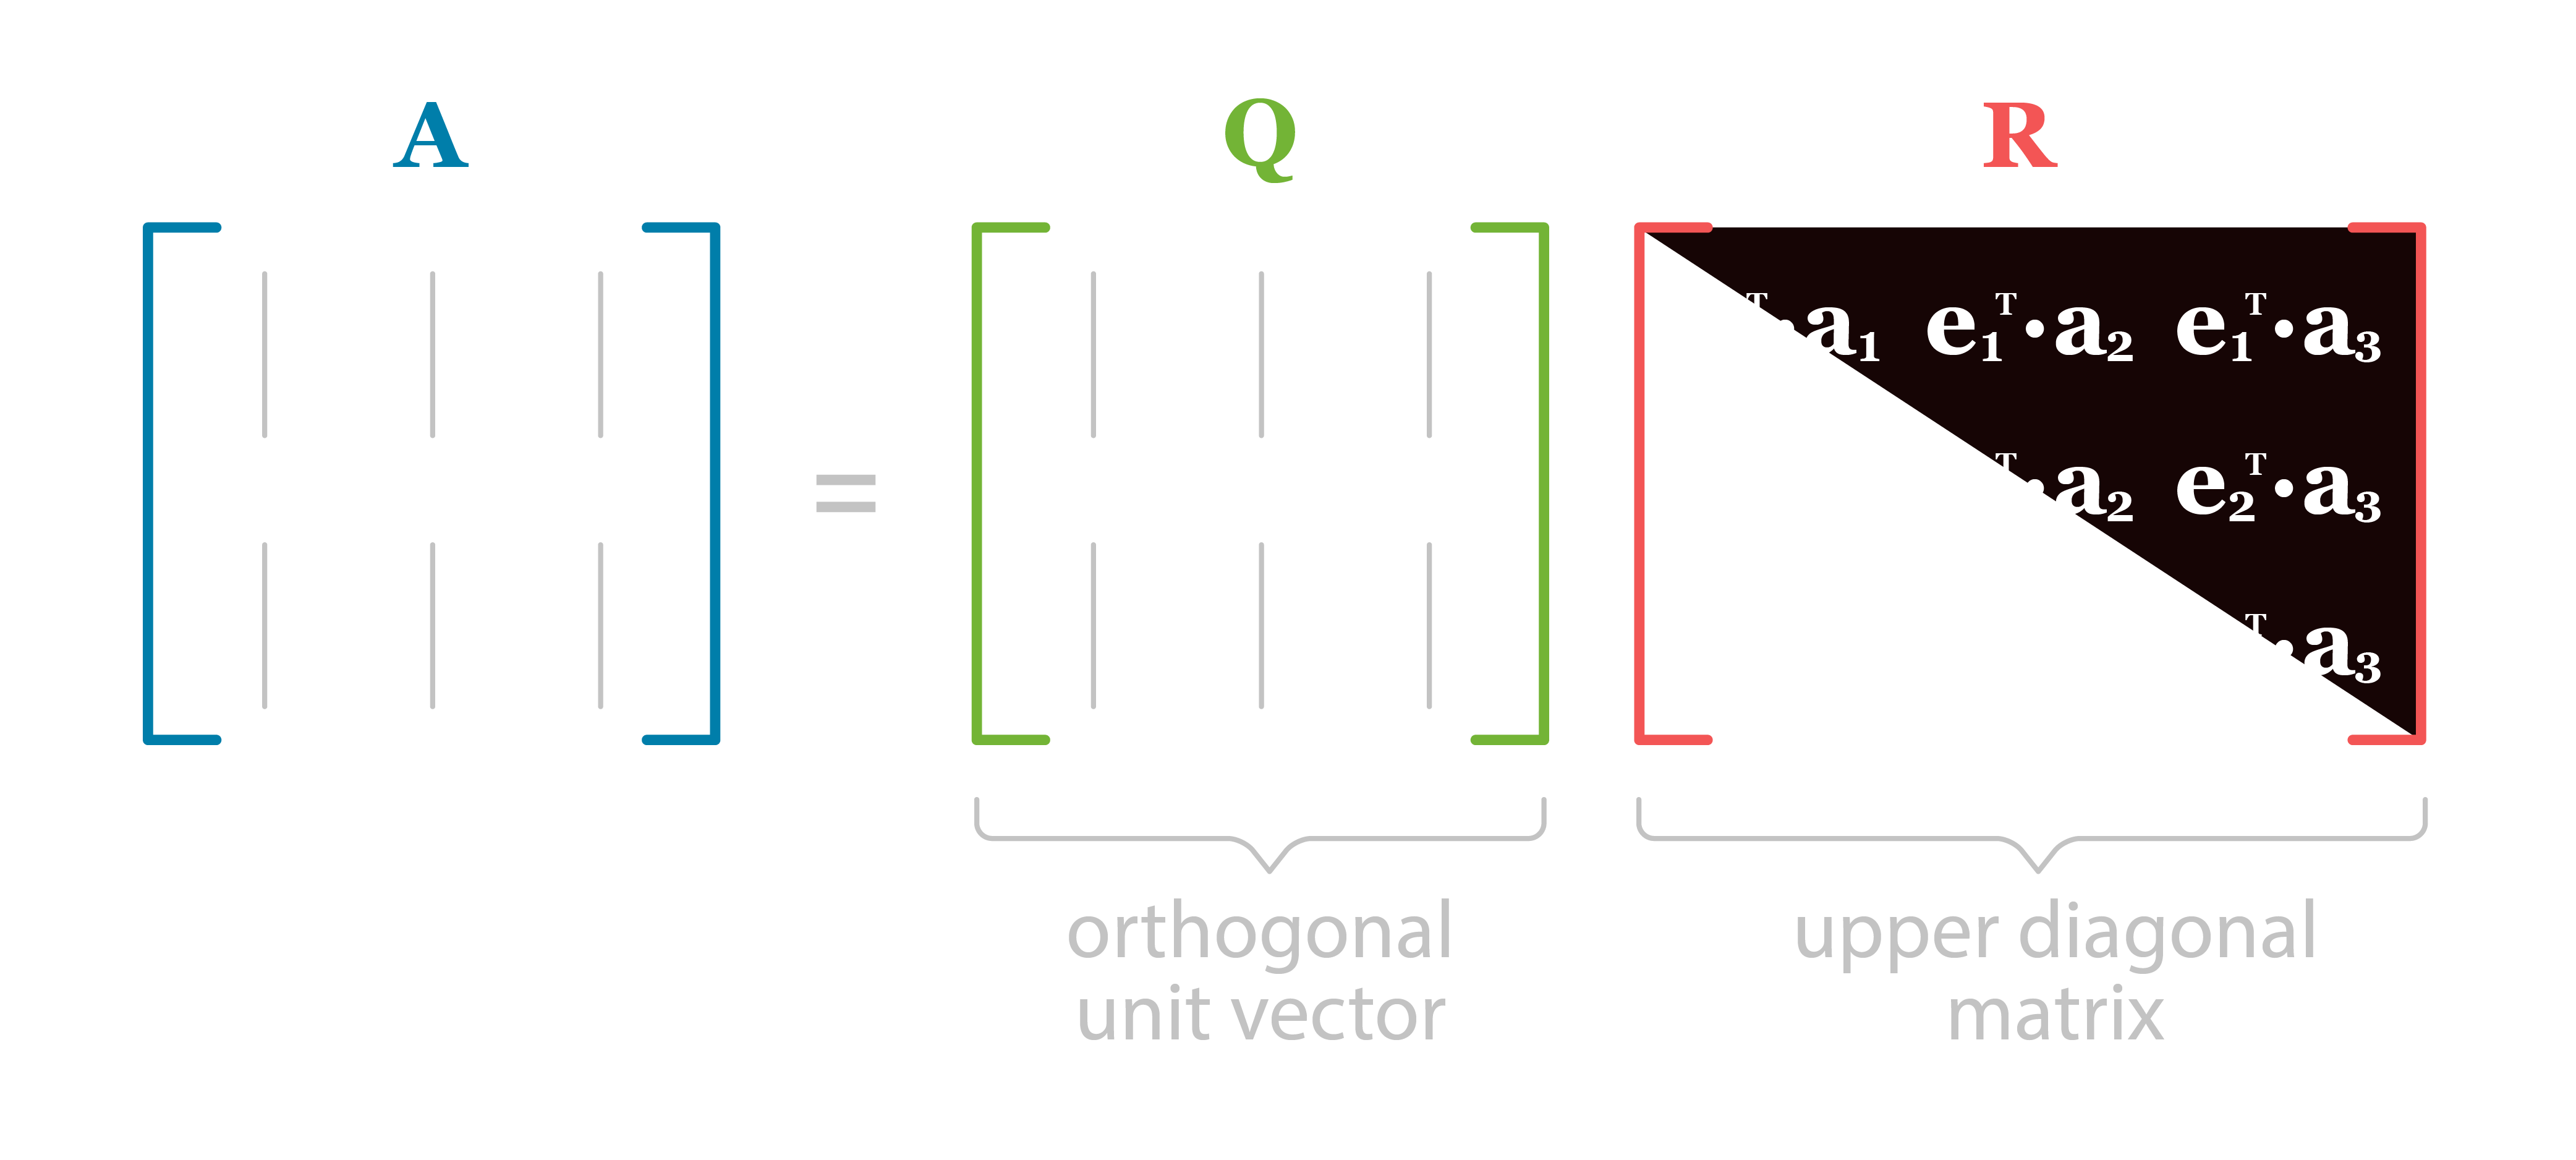
\includegraphics[scale=0.2]{./figures/QR-neg.png} \end{center}
}
%-------------- end slide -------------------------------%}}}
%-------------- start slide -----------------------------% {{{ 4
\frame{
\begin{theorem}
    Let $A$ be a real $m \times n$ matrix with linearly independent columns. Then $A$ can be written
    \[
	A = QR
    \]
    with $Q$ orthogonal and $R$ upper triangular with positive entries on the main diagonal.
\end{theorem}
\vfill
\pause
\begin{proofnoend}
    Using columns of $A$ to carry out the Gram-Schmidt algorithm to find an orthonormal basis for $\im(A)$ or $\col(A)\subseteq\R^m$ -- columns of $Q_1$.
    One may further extend this basis to an orthonormal basis for the whole space $\R^m$ -- columns of $Q = [Q_1,Q_2]$.
    \begin{center}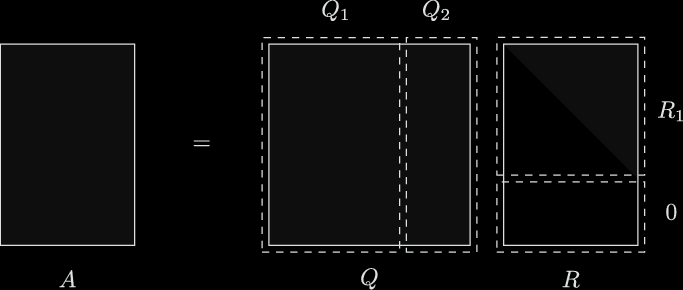
\includegraphics[scale=0.25]{./figures/QR2-neg.png} \end{center}
    The Gram-Schmidt algorithm guarantees that the $i$th column of $A$ is linear combinations of all $j$th columns of $Q$ with $j=1,\cdots, i$,
    which gives the upper triangular structure of $R$.
    \myQED
\end{proofnoend}
}
%-------------- end slide -------------------------------%}}}
%-------------- start slide -----------------------------% {{{ 5
\frame{
\begin{center}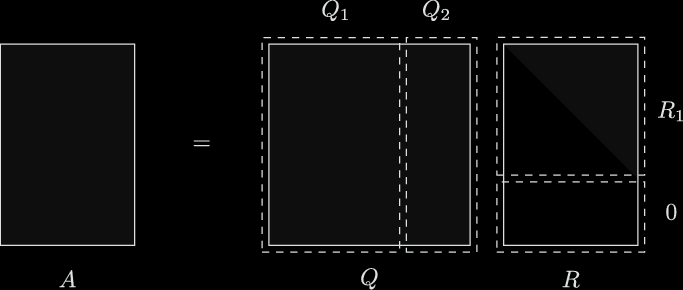
\includegraphics[scale=0.25]{./figures/QR2-neg.png} \end{center}
\vfill
\begin{remark}
   \begin{align*}
       A = Q R  = [Q_1,Q_2] \begin{bmatrix} R_1\\ O \end{bmatrix} = Q_1 R_1 + Q_2 O = Q_1 R_1.
   \end{align*}
   Both $QR$ and $Q_1R_1$ are called QR decompositions of $A$. The textbook refers $Q_1R_1$.
\end{remark}
\vfill
\begin{remark}
   $Q$ is orthogonal matrix, namely, $Q Q^T = Q^TQ = I_m$. \\
   However, $Q_1$ is not orthogonal matrix (not a square matrix). But We have
   $Q_1^TQ_1=I_n$ and $Q_1Q_1^T\ne I_m$ (in general).
\end{remark}
}
%-------------- end slide -------------------------------%}}}
\section[\textcolor{yellow}{}]{\textcolor{yellow}{Algorithm for the QR Factorization}}
%-------------- start slide -----------------------------% {{{ 6
\frame{
\begin{emptytitle}
\frametitle{Algorithm for QR Factorization}
\pause
\begin{center}
    \begin{minipage}{0.95\textwidth}
	\begin{algorithm*}[H]
	    \SetKwInOut{Input}{Input}\SetKwInOut{Output}{Output}
	    \Input{Independent columns of $A$:  $\{ \vec{c}_1, \vec{c}_2, \ldots, \vec{c}_n\}\in \col(A)\subseteq \R^m$}
	    \BlankLine
	    \SetAlgoLined
	     \For{$j\leftarrow 1$ \KwTo $n$}{
	       \[
		    \vec{f}_j\leftarrow \vec{c}_j
		    -\frac{\vec{c}_j\dotprod\vec{f}_1}{||\vec{f}_1||^2}\vec{f}_1
		    -\frac{\vec{c}_j\dotprod\vec{f}_2}{||\vec{f}_2||^2}\vec{f}_2 -\cdots
		    -\frac{\vec{c}_j\dotprod\vec{f}_{j-1}}{||\vec{f}_{j-1}||^2}\vec{f}_{j-1}.
	       \]
	       \[
		    \vec{q}_j \leftarrow \frac{\vec{f}_j}{||\vec{f}_j||}
	       \]
		 \For{$i\leftarrow 1$ \KwTo $j$}{
		   \[
		       r_{ij} \leftarrow \vec{q}_i \cdot \vec{c}_j
		   \]
		   }
	       }
	       \Output{$Q=[\vec{q}_1,\cdots,\vec{q}_n]$ and $R=[r_{ij}]$}
	\caption{QR Factorization Algorithm}
    \end{algorithm*}
    \end{minipage}
\end{center}
\end{emptytitle}
}
%-------------- end slide -------------------------------%}}}
%-------------- start slide -------------------------------%{{{ --
% \begin{frame}[fragile]
%  \begin{emptytitle}
%     Let $A$ be a real $m \times n$ matrix with linearly independent columns $A_1, A_2, \cdots, A_n$. The following procedure results in the $QR$ factorization.
%     \medskip
%     \pause
%
%     \begin{enumerate}
% 	\item    Apply the Gram-Schmidt Process to the columns of $A$. Label the resulting columns $B_1, B_2, \cdots, B_n$ respectively.
% 	\item    Define $C_i = \frac{1}{|| B_i ||} B_i$.
% 	\item    Let $Q$ be constructed as $Q = \leftB \begin{array}{cccc}
% 	C_1 & C_2 & \cdots & C_n \end{array}\rightB$. Then $Q$ is orthogonal.
% 	\item    Let $R$ be constructed as
% 	\[
% 	R = \leftB \begin{array}{ccccc}
% 	    || B_1 || & A_2 \dotprod C_1 & A_3 \dotprod C_1 & \cdots & A_n \dotprod C_1 \\
% 	    0         & || B_2 ||        & A_3 \dotprod C_2 & \cdots & A_n \dotprod C_2 \\
% 	    0         & 0                & || B_3 ||        & \cdots & A_n \dotprod C_1 \\
% 	    \vdots    & \vdots           & \vdots           &        & \vdots           \\
% 	    0         & 0                & 0                & \cdots & || B_n ||
% 	\end{array}\rightB
% 	\]
% 	\item    The result is $A = QR$.
%     \end{enumerate}
% \end{emptytitle}
% \end{frame}
%-------------- end slide -------------------------------%}}}
%-------------- start slide -----------------------------% {{{ 7
\frame{
\begin{problem}
    Let
    \[
    A = \leftB \begin{array}{rr}
	4 & 1 \\
	2 & 3 \\
	0 & 1
    \end{array}\rightB
    \]
    Find the $QR$ factorization of $A$.
\end{problem}
\vfill
\pause
\begin{solution}
    Set $A=[\vec{c}_1,\vec{c}_2]$.
    When $j=1$,
    \begin{align*}
	\vec{f} _1 &= \vec{c} _1 = \leftB \begin{array}{r} 4 \\ 2 \\ 0 \end{array} \rightB \quad\text{and}\quad
	\vec{q}_1 = \frac{\vec{f}_1}{||\vec{f}_1||}  = \begin{bmatrix} \frac{4}{\sqrt{20}}\\ \frac{2}{\sqrt{20}}\\ 0 \end{bmatrix}.
    \end{align*}
   For $i=1$,
   \begin{align*}
       r_{11} = \vec{q}_1\cdot \vec{c}_1  = \frac{\vec{f}_1}{||\vec{f}_1||}\cdot \vec{f}_1 = ||\vec{f}_1|| = \sqrt{20}.
   \end{align*}
\end{solution}
}
%-------------- end slide -------------------------------%}}}
%-------------- start slide -----------------------------% {{{ 8
\frame{
\begin{solution}[continued]
    When $j=2$,
    \begin{align*}
	\vec{f} _2 &= \vec{c} _2 - \frac{\vec{c}_2\cdot \vec{f}_1}{||\vec{f}_1 ||^2}\vec{f}_1  = \leftB \begin{array}{r} 1 \\ 3 \\ 1 \end{array} \rightB - \frac{10}{20} \leftB \begin{array}{r} 4 \\ 2 \\ 0 \end{array} \rightB = \leftB \begin{array}{r} -1 \\ 2 \\ 1 \end{array} \rightB
	\quad\text{and}\quad
	\vec{q}_2 = \frac{\vec{f}_2}{||\vec{f}_2||}  = \begin{bmatrix} -\frac{1}{\sqrt{6}}\\ \frac{2}{\sqrt{6}}\\ \frac{1}{\sqrt{6}} \end{bmatrix}.
    \end{align*}
    For $i=1$,
   \begin{align*}
       r_{12} = \vec{q}_1\cdot \vec{c}_2  = \begin{bmatrix} \frac{4}{\sqrt{20}}\\ \frac{2}{\sqrt{20}}\\ 0 \end{bmatrix} \cdot \begin{bmatrix} 1\\ 3\\ 1 \end{bmatrix}  = \sqrt{5}.
   \end{align*}
   and for $i=2$,
   \begin{align*}
       r_{22} = \vec{q}_2\cdot \vec{c}_2  = \frac{\vec{f}_2}{||\vec{f}_2||}\cdot \left(\vec{f}_2+\frac{\vec{c}_2\cdot \vec{f}_1}{||\vec{f}_1 ||^2}\vec{f}_1\right) =
       \frac{\vec{f}_2}{||\vec{f}_2||}\cdot \vec{f}_2 = ||\vec{f}_2|| = \sqrt{6}.
   \end{align*}
\end{solution}
}
%-------------- end slide -------------------------------%}}}
%-------------- start slide -----------------------------% {{{ 9
\frame{
\begin{solution}[continued]
Therefore,
\begin{align*}
    A = QR  = [\vec{q}_1, \vec{q}_2]
	\begin{bmatrix}
	    r_{11} & r_{12} \\
	    0      & r_{22} \\
	\end{bmatrix}
\end{align*}
\[\Updownarrow\]
\begin{align*}
    \leftB \begin{array}{rr}
	4 & 1 \\
	2 & 3 \\
	0 & 1
    \end{array}\rightB = \leftB \begin{array}{rr}
    \frac{2}{\sqrt{5}} & -\frac{1}{\sqrt{6}} \\
    \frac{1}{\sqrt{5}} & \frac{2}{\sqrt{6}}  \\
    0                  & \frac{1}{\sqrt{6}}
    \end{array}\rightB \leftB \begin{array}{ccccc}
    \sqrt{20} & \sqrt{5} \\
    0         & \sqrt{6} \\
    \end{array}\rightB
\end{align*}
\myQED
\end{solution}
}
%-------------- end slide -------------------------------%}}}
\end{document}
